\documentclass[11pt]{beamer}
\usepackage[utf8]{inputenc}
\usepackage[T1]{fontenc}
\usepackage{amsmath}
\usepackage{amsfonts}
\usepackage{amssymb}
\usepackage{graphicx}
\usetheme{default}

\begin{document}
	\author{Musa Baloyi}
	\title{Application performance monitoring}
	%\subtitle{Model governance for risk management}
	%\logo{}
	%\titlegraphic{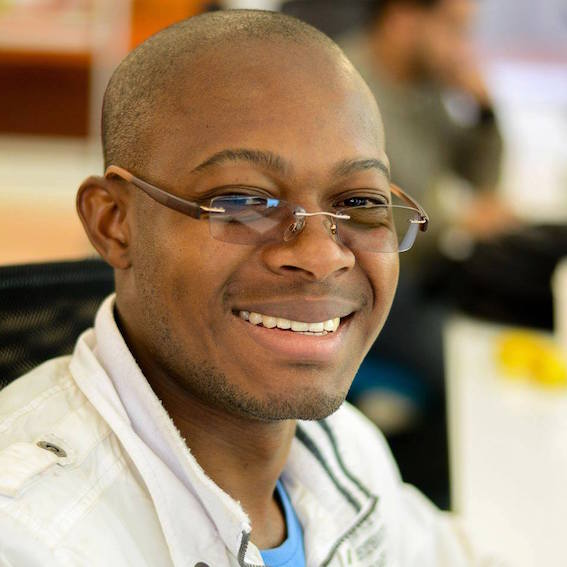
\includegraphics[width=\textwidth,height=.5\textheight]{logo}}
	%\institute{}
	%\date{}
	%\subject{}
	%\setbeamercovered{transparent}
	%\setbeamertemplate{navigation symbols}{}
	\begin{frame}[plain]
	\maketitle
\end{frame}

\begin{frame}
\frametitle{Table of contents}
\begin{itemize}
	\item Traditional application performance monitoring
	\item Machine learning model monitoring
	\item Data generation
	\begin{itemize}
		\item Out of the box logging
		\item Custom logging
		\item Data dictionaries
		\item Data types
		\item File types
	\end{itemize}
	\item Data movement primer (Kafka)
	\item Data transformation primer (Logstash)
	\item Data visualisation primer (Kibana)
	\item Next steps: application performance management
\end{itemize}
\end{frame}


\begin{frame}
\frametitle{Logging facility for Python}
\begin{itemize}
\item This module defines functions and classes which implement a flexible event logging system for applications and libraries.
\item The key benefit of having the logging API provided by a standard library module is that all Python modules can participate in logging, so your application log can include your own messages integrated with messages from third-party modules.
\end{itemize}
\end{frame}


\begin{frame}
\frametitle{Logging facility for Python}
The basic classes defined by the module, together with their functions, are:
\begin{itemize}
	\item Loggers expose the interface that application code directly uses.
	\item Handlers send the log records (created by loggers) to the appropriate destination.
	\item Filters provide a finer grained facility for determining which log records to output.
	\item Formatters specify the layout of log records in the final output.
\end{itemize}
\end{frame}

\begin{frame}
\frametitle{Logging facility for Python}
Logging serves two purposes:
\begin{itemize}
	\item Diagnostic logging records events related to the application’s operation. If a user calls in to report an error, for example, the logs can be searched for context.
	\item Audit logging records events for business analysis. A user’s transactions can be extracted and combined with other user details for reports or to optimize a business goal.
\end{itemize}
\end{frame}


\begin{frame}
\frametitle{dsds\_logging guide}
\begin{enumerate}
	\item git clone https://<username>@tools.standardbank.co.za/bitbucket/scm/datas/python-packages.git
	\item sys.path.append("../python-packages/dsds")
	\item import dsds.dsds\_logging
	\item config, logger = dsds\_spark.get\_config\_and\_logger(sys.argv)
	\item sc, hiveContext = dsds\_spark.get\_contexts(config, sys.argv)
	\item spark\_main(config, logger, sc, hiveContext)
	\item logger.info('Feature\_extraction.py', 'feature\_set\_6', feature\_set\_6.columns)
\end{enumerate}
\end{frame}


\begin{frame}
\frametitle{Sample log (.txt)}
\begin{figure}[h]
	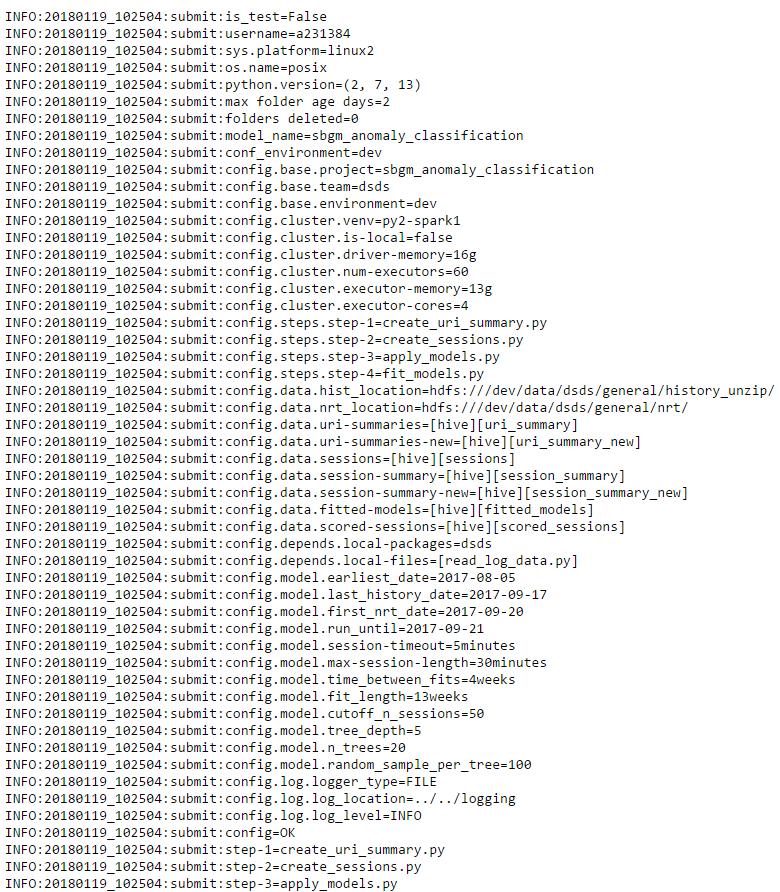
\includegraphics[scale=.35]{images/txt_log}
\end{figure}
\end{frame}


\begin{frame}
\frametitle{Sample log (.json)}
\begin{figure}[h]
	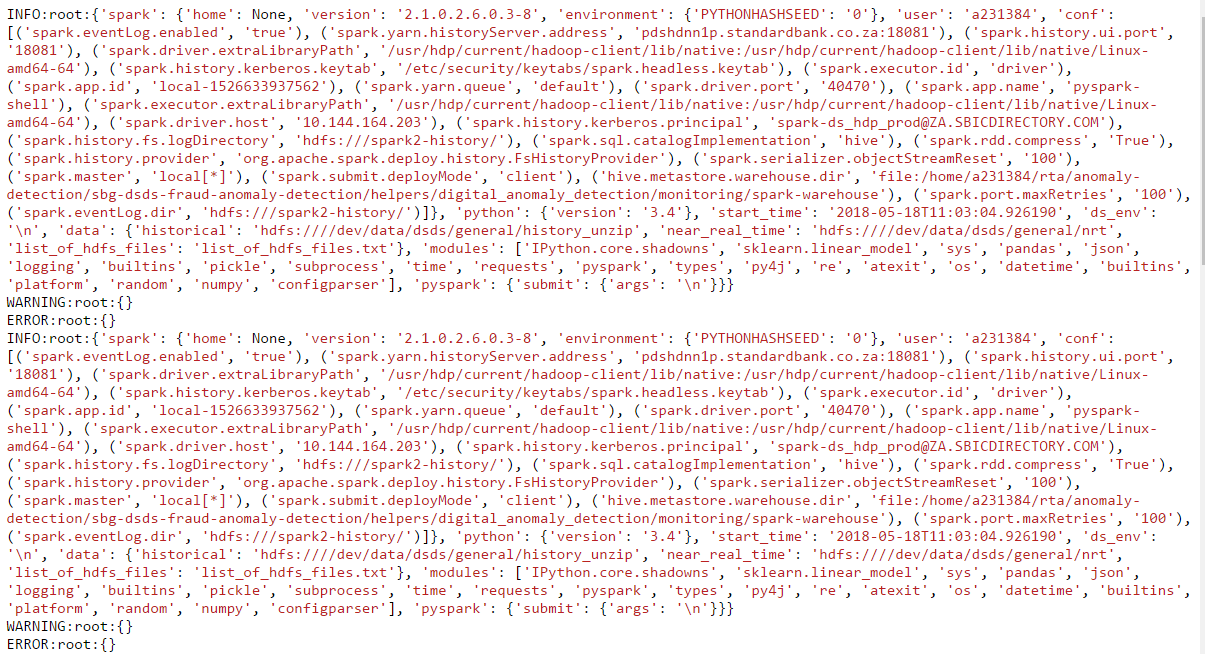
\includegraphics[scale=.35]{images/json_log}
\end{figure}
\end{frame}


\begin{frame}
\frametitle{Monitoring}
\begin{itemize}
	\item Managing and monitoring statistical models is crucial if your organization periodically runs a large number (say, over 10) of statistical models. 
	\item However, these issues are important even when there are just a few of them in production. 
\end{itemize}
\end{frame}


\begin{frame}
\frametitle{Monitoring}
Common challenges include the following: 
\begin{itemize}
	\item Keeping all the input correct and fresh. 
	\item Making sure the outputs go to the right places, in the correct formats. 
	\item Keeping the code organized for effective updating and maintenance. 
	\item Creating and maintaining effective documentation. 
	\item Assessing and tracking model performance. 
	\item Effectively (preferably automatically) deciding when to update the model.
\end{itemize}
\end{frame}


\begin{frame}
\frametitle{Monitoring: all models}
\begin{itemize}
	\item Model: name.
	\item Environment: continuous development and integration; software and versions; hardware statistics; environment variables; run mode; current build version; source and run location; steps; extra packages and files; run command.
	\item Data: historical location; near real-time location; maximum folder age; logs start and end date; last history date; model last date; next run date; first NRT date.
	\item Results: submit status; total runtime; FLS alerts; loglines.
\end{itemize}
\end{frame}


\begin{frame}
\frametitle{Monitoring: supervised models}
\begin{itemize}
	\item Statastical process control: drift detection method (DDM); early drift detection method (EDDM).
	\item Sequential analysis: linear four rates (true –ve, false –ve, true +ve, false +ve) – specificity, recall, precision, accuracy; Monte Carlo sampling for significance level; Bonferoni correction for correlated tests.
	\item Error distribution monitoring: adaptive windowing (ADWIN)
\end{itemize}
\end{frame}


\begin{frame}
\frametitle{Monitoring: unsupervised models}
\begin{itemize}
	\item Clustering/novelty detection
	\item Feature distribution monitoring
	\item Model-dependent monitoring
\end{itemize}
\end{frame}


\begin{frame}
\frametitle{Monitoring: random forests}
\begin{itemize}
	\item Number of URI’s
	\item Time between fits
	\item Samples per tree
	\item Model start date
	\item Number of sessions to score
	\item Previous run date
	\item Maximum session length
	\item Last URI timestamp
\end{itemize}
\end{frame}


\begin{frame}
\frametitle{Monitoring: k-means}
\begin{itemize}
	\item Database name
	\item Results
	\item Alerts to FLS
	\item Model path
	\item List of features
	\item Clusters
\end{itemize}
\end{frame}


\begin{frame}
\frametitle{Visualisation}
\begin{figure}[h]
	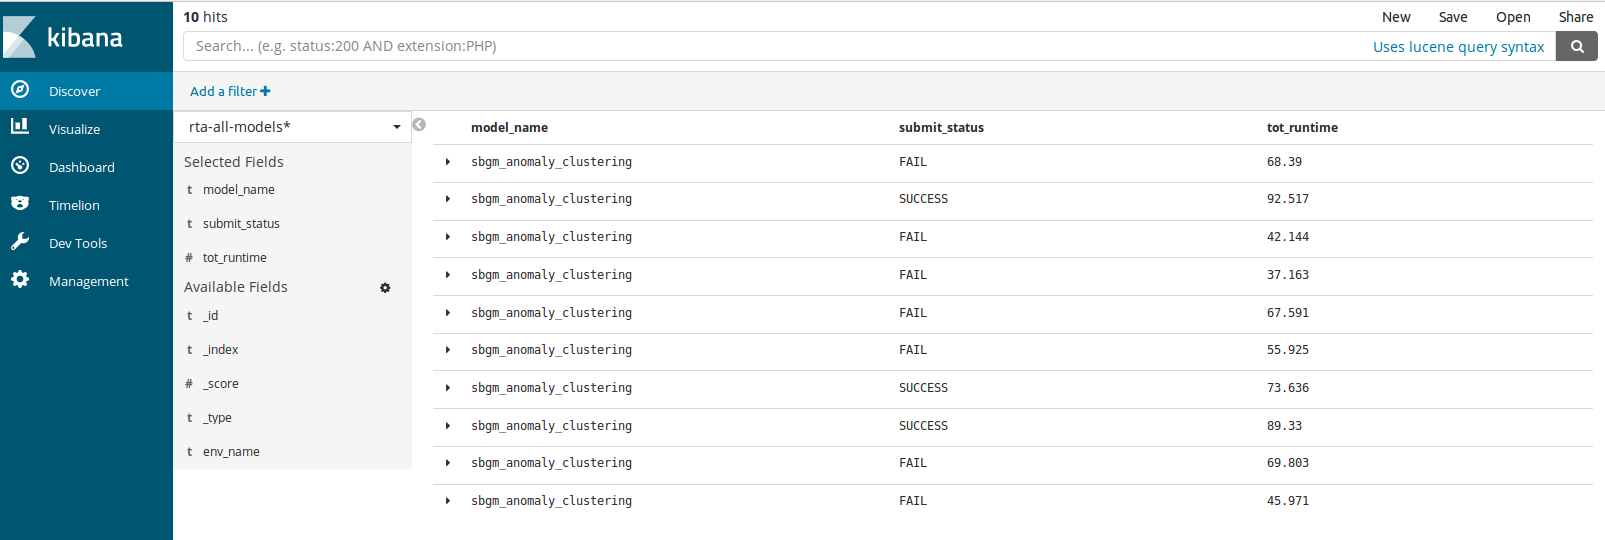
\includegraphics[scale=.2]{images/viz1}
\end{figure}
\end{frame}


\begin{frame}
\frametitle{References}
\begin{enumerate}
	\item Building Intelligent Systems: A Guide to Machine Learning Engineering. [Geoff Hulten] (Apress, 2018)
	\item Trends in AI, Data Science, and Big Data. [Ben Lorica] (2017)
	\item Building Evolutionary Architectures. [Rebecca Parsons; Patrick Kua; Neal Ford] (O'Reilly Media, 2017)
	\item 5 things you should be monitoring. [Brian Brazil] (2018)
	\item The Logstash Book. [James Turnbull] (Turnbull Press, 2013)
	\item Beyond the Twelve-Factor App. [Kevin Hoffman] (O'Reilly Media, 2016)
	\item Logs and real-time stream processing. [Jay Kreps] (2016)
	\item I Heart Logs: Apache Kafka and Real-time Data Integration. [Jay Kreps] (2015)
	\item The log: The lifeblood of your data pipeline. [Kiyoto Tamura] (2015)
	\item Understanding the ELK stack. [Brian Anderson; Rafał Kuć] (2016)
\end{enumerate}
\end{frame}

\end{document}